
\titledquestion{Tree Surgery and Traversal}

The following ordered rooted tree $T$ has root $R$
(children are listed from left to right).
The height of a tree is measured in edges.

\makebox[\textwidth][c]{
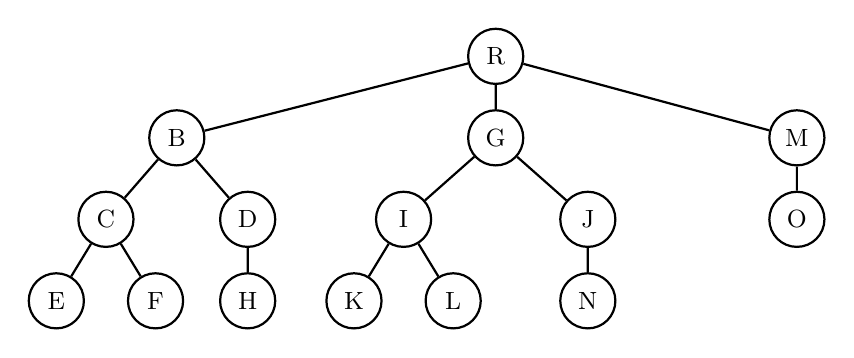
\begin{tikzpicture}[
    thick,
    scale=0.9,
    every node/.style={
        circle,
        draw,
        minimum size=7mm,
        inner sep=1pt,
        font=\small
    }
]
    % Root
    \node (R) at (0,0) {R};

    % Depth 1
    \node (B) at (-4.5,-1.15) {B};
    \node (G) at (0,-1.15) {G};
    \node (M) at (4.25,-1.15) {M};

    % Depth 2
    \node (C) at (-5.5,-2.3) {C};
    \node (D) at (-3.5,-2.3) {D};
    \node (I) at (-1.3,-2.3) {I};
    \node (J) at (1.3,-2.3) {J};
    \node (O) at (4.25,-2.3) {O};

    % Depth 3
    \node (E) at (-6.2,-3.45) {E};
    \node (F) at (-4.8,-3.45) {F};
    \node (H) at (-3.5,-3.45) {H};
    \node (K) at (-2.0,-3.45) {K};
    \node (L) at (-0.6,-3.45) {L};
    \node (N) at (1.3,-3.45) {N};

    % Edges
    \draw
        (R)--(B)
        (R)--(G)
        (R)--(M)
        (B)--(C)
        (B)--(D)
        (C)--(E)
        (C)--(F)
        (D)--(H)
        (G)--(I)
        (G)--(J)
        (I)--(K)
        (I)--(L)
        (J)--(N)
        (M)--(O);
\end{tikzpicture}
}

\medskip

Perform the following operations \textbf{in this order}:

\begin{enumerate}
    \item Detach the entire subtree rooted at $I$ from $G$,
    then attach it as the \textbf{rightmost child} of $D$.

    \item Detach the entire subtree rooted at $C$ from $B$,
    then attach it as the \textbf{leftmost child} of $M$.
\end{enumerate}

For the resulting tree, answer the following questions.

\begin{parts}

    %%%%%%%%%%%%%%%%%%%%%%%%%%%%%%%%%%%%%%%%%%%%%%%%%%%%%%%%%%
    % (a) Tree Surgery
    % 4 points
    %%%%%%%%%%%%%%%%%%%%%%%%%%%%%%%%%%%%%%%%%%%%%%%%%%%%%%%%%%

    \part[4] Draw the resulting ordered tree,
    showing every node and edge.

    \begin{solution}
        
        \makebox[\textwidth][c]{
        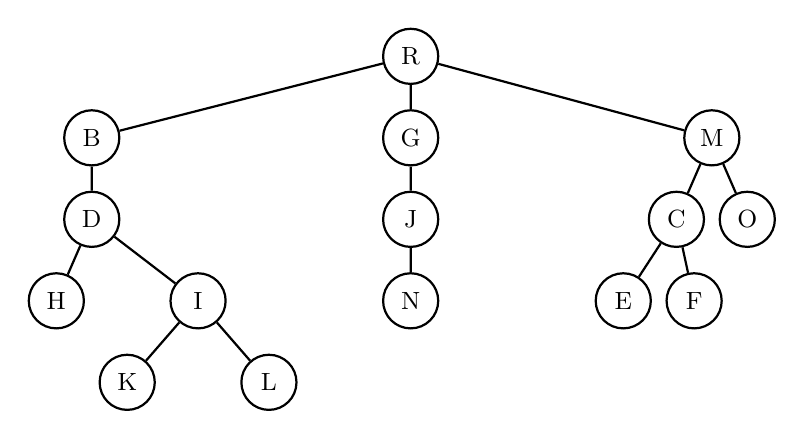
\begin{tikzpicture}[
            thick,
            scale=0.9,
            every node/.style={
                circle,
                draw,
                minimum size=7mm,
                inner sep=1pt,
                font=\small
            }
        ]
            % Root
            \node (R) at (0,0) {R};

            % Depth 1
            \node (B) at (-4.5,-1.15) {B};
            \node (G) at (0,-1.15) {G};
            \node (M) at (4.25,-1.15) {M};

            % Depth 2
            \node (D) at (-4.5,-2.3) {D};
            \node (J) at (0,-2.3) {J};
            \node (C) at (3.75,-2.3) {C};
            \node (O) at (4.75,-2.3) {O};

            % Depth 3
            \node (H) at (-5.0,-3.45) {H};
            \node (I) at (-3.0,-3.45) {I};
            \node (N) at (0,-3.45) {N};
            \node (E) at (3.0,-3.45) {E};
            \node (F) at (4.0,-3.45) {F};

            % Depth 4
            \node (K) at (-4.0,-4.6) {K};
            \node (L) at (-2.0,-4.6) {L};

            % Edges
            \draw
                (R)--(B)
                (R)--(G)
                (R)--(M)
                (B)--(D)
                (C)--(E)
                (C)--(F)
                (D)--(H)
                (D)--(I)
                (G)--(J)
                (I)--(K)
                (I)--(L)
                (J)--(N)
                (M)--(O)
                (M)--(C);
        \end{tikzpicture}
        }

        \medskip
    \end{solution}


    %%%%%%%%%%%%%%%%%%%%%%%%%%%%%%%%%%%%%%%%%%%%%%%%%%%%%%%%%%
    % (b) Height and Subtree Size
    % 2 points: 1 + 1
    %%%%%%%%%%%%%%%%%%%%%%%%%%%%%%%%%%%%%%%%%%%%%%%%%%%%%%%%%%

    \part[2] Give the \textbf{height} of the resulting
    tree and the \textbf{size} of the subtree rooted at $D$.

    \begin{solution}
        height = 4, size of subtree rooted at D = 5
    \end{solution}


    %%%%%%%%%%%%%%%%%%%%%%%%%%%%%%%%%%%%%%%%%%%%%%%%%%%%%%%%%%
    % (c) Traversal Sequences
    % 2 points: 1 + 1
    %%%%%%%%%%%%%%%%%%%%%%%%%%%%%%%%%%%%%%%%%%%%%%%%%%%%%%%%%%

    \part[2] Give both the \textbf{preorder DFS}
    and \textbf{BFS} traversal sequences of the
    resulting tree. Children are processed
    from left to right.

    \begin{solution}

        Preorder DFS: R, B, D, H, I, K, L, G, J, N, M, C, E, F, O

        BFS: R, B, G, M, D, J, C, O, H, I, N, E, F, K, L
    \end{solution}


    %%%%%%%%%%%%%%%%%%%%%%%%%%%%%%%%%%%%%%%%%%%%%%%%%%%%%%%%%%
    % (d) Stack State During DFS
    % 2 points
    %%%%%%%%%%%%%%%%%%%%%%%%%%%%%%%%%%%%%%%%%%%%%%%%%%%%%%%%%%

    \part[2] Perform \textbf{preorder DFS} on the
    resulting tree using a \textbf{stack}.
    Initially, push the root onto the stack.
    When a node is popped, push its children
    in \textbf{reverse order} (right to left),
    so that children are visited left to right.

    Immediately after node $D$ is popped and
    its children are pushed, list the
    \textbf{entire stack from bottom to top}.

    \begin{solution}
        
        Initial stack: R

        Pop R, push M, G, B (stack: M, G, B)

        Pop B, push D (stack: M, G, D)

        Pop D, push I, H (stack: M, G, I, H)

        Stack from bottom to top: M, G, I, H
    \end{solution}

\end{parts}
